% 
% Annual Cognitive Science Conference
% Sample LaTeX Paper -- Proceedings Format
% 

% Original : Ashwin Ram (ashwin@cc.gatech.edu)       04/01/1994
% Modified : Johanna Moore (jmoore@cs.pitt.edu)      03/17/1995
% Modified : David Noelle (noelle@ucsd.edu)          03/15/1996
% Modified : Pat Langley (langley@cs.stanford.edu)   01/26/1997
% Latex2e corrections by Ramin Charles Nakisa        01/28/1997 
% Modified : Tina Eliassi-Rad (eliassi@cs.wisc.edu)  01/31/1998
% Modified : Trisha Yannuzzi (trisha@ircs.upenn.edu) 12/28/1999 (in process)
% Modified : Mary Ellen Foster (M.E.Foster@ed.ac.uk) 12/11/2000
% Modified : Ken Forbus                              01/23/2004
% Modified : Eli M. Silk (esilk@pitt.edu)            05/24/2005
% Modified: Niels Taatgen (taatgen@cmu.edu) 10/24/2006

%% Change ``a4paper'' in the following line to ``letterpaper'' if you are
%% producing a letter-format document.

\documentclass[10pt,letterpaper]{article}

\usepackage{cogsci}
\usepackage{pslatex}
\usepackage{graphicx}
\usepackage{wrapfig}
\usepackage{subcaption}
\usepackage{algorithm}
\usepackage{algpseudocode}
\usepackage[
backend=biber,
sorting=ynt
]{biblatex}
\bibliography{references.bib}
\addbibresource{references.bib}

\title{Exploring and exploiting Monte-Carlo Othello}

\author{\large \bf Richard Deurwaarder}

\begin{document}

\maketitle

\begin{abstract}
The abstract should be one paragraph, indented 1/8~inch on both sides,
in 9~point font with single spacing. The heading {\bf Abstract} should
be 10~point, bold, centered, with one line space below it. This
one-paragraph abstract section is required only for standard spoken
papers and standard posters (i.e., those presentations that will be
represented by six page papers in the Proceedings).
n
\end{abstract}

\section{Introduction}
Monte Carlo planning has long been a good solution to find near optimal solutions to large state space Markovian Decision Problems. This is a type of problem where an action needs to be taken to stochastically move to a new state which will give some kind of reward, this reward needs to be optimized. When the problems become sufficiently large it quickly becomes infeasible to search the whole space and trade-offs need to be made. In this paper I will look at the board game Othello in particular.\\

Because of the large state space it is useful to gather information about which actions are more promising than other, and put more effort into investigating states which are a result of those actions. This is the classic exploration versus exploitation problem: How much effort do we put into exploring how promising the actions are and how much effort is put into exploiting these actions. One algorithm proposed by Kocsis and Szepesvari\cite{Kocsis:2006} called UCT deals with this problem.

UCT has a parameter called the exploration parameter. This determines how likely or unlikely the algorithm is to explore or exploit. In practice this parameter is chosen without too much consideration. In this paper I will try to show the significance of this parameter for the game Othello.

\subsection{Othello}
Othello is a strategy board game for two players. Sometimes also referred to as Reversi. Players are assigned a color and take turns placing pieces on the board while capturing pieces of the other player. The player with most pieces left at the end of the game wins. 
\subsubsection{Board and moves}
Othello is played on a 8x8 uncheckered board. It always has the same starting position, see figure: \ref{fig:othello-startposition}. Making a move is done by placing a piece on an empty square and capturing at least one piece of the opponent in the process. A piece is captured when it becomes surrounded by the other color, see figure: \ref{fig:othello-capture}. When white places a piece on F3. Five pieces get captured and turn white. However E5 does not get captured because it does not get surrounded by F3, it only gets surrounded via the effects of F3.
\subsubsection{Importance of different squares} The pieces in the middle of the board might be captured and recaptured multiple times, because they are surrounded by so many different positions but note the corner squares will never be captured once initially filled, because they cannot be surrounded, making it a safe and valuable position to take.
\subsubsection{Game results} The winner of the game is determined by the player with the most pieces at the end of the game. The game ends is when no other available moves are left, this might happen before all the squares are filled, because you may only place a piece if you capture at least one other. It does not matter by how many pieces you you beat the opponent.


\begin{figure}
    \centering
    \begin{subfigure}{0.25\textwidth}
        \caption{Start position}
        \label{fig:othello-startposition}
        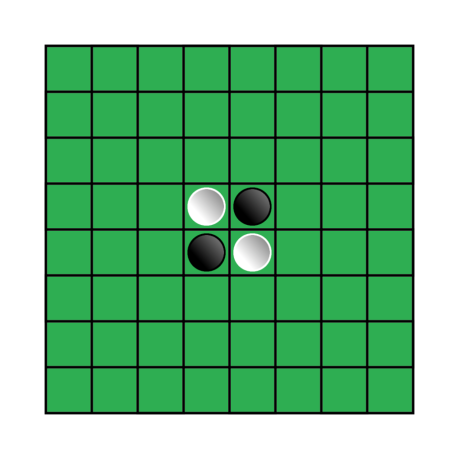
\includegraphics[width=\textwidth]{images/startposition}
    \end{subfigure}%
    \begin{subfigure}{.25\textwidth}
        \caption{White captures}
        \label{fig:othello-capture}
        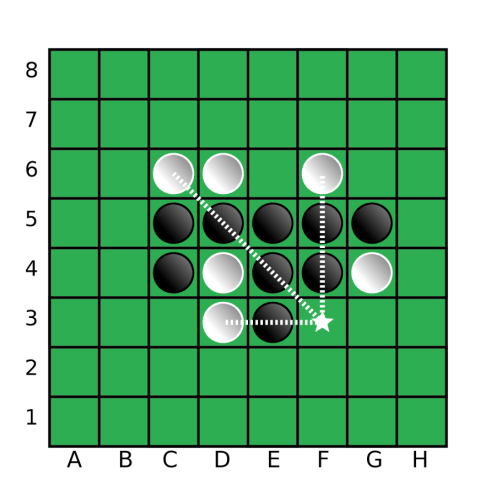
\includegraphics[width=\textwidth]{images/capture}
    \end{subfigure}
    \caption{Uncheckered 8x8 boards}
\end{figure}

\begin{figure}
    \centering
    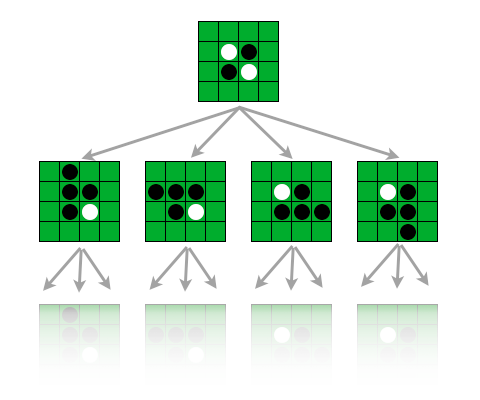
\includegraphics[width=0.4\textwidth]{images/othello-gametree}
    \caption{Othello tree representation}
    \label{fig:othello-gametree}
\end{figure}
\subsection{Monte Carlo Tree search}
\subsubsection{Tree search}
A game of Othello can be represented as a tree structure where each node represents the state of the board with all its pieces and each edge being a valid action that can be taken to transition from one node to the other. See figure \ref{fig:othello-gametree}. Leafs in the tree would be terminating states, for instance when the board as been completely filled with pieces. Tree structures like these can be called game trees. Searching through these game trees and finding a (near) optimal move to make can be achieved via different algorithms.

\subsubsection{Minimax tree}
Minimax is a way to search through a game tree and find a good action in a turn based game such as Othello. It works under the assumption that the opponent will always try to win by making optimal moves (minimizing the score of the player while maximizing its own). Figure \ref{fig:mcts-gametree-values} shows a game tree with some values per node. The values for each node indicate how well this node is for the players. In fig \ref{fig:mcts-gametree-values} the white nodes indicate that it's the first player's turn to move, the gray nodes are when it is the second player's turn. Player 1 will choose actions that will maximize it's own score, while player 2 will choose actions that minimizes the score of player 1.

\begin{algorithm}
\caption{Monte Carlo Tree Search}
\label{algo:mcts}
\begin{algorithmic}
\Function{MonteCarloPlanning}{rootNode}
\While{no timeout}
\State $leafNode \gets \Call{Select}{rootNode}$
\State $(action, newNode) \gets \Call{Expand}{leafNode}$
\State $reward \gets \Call{Simulate}{newNode}$
\State $ancestors \gets \Call{getAncestors}{newNode}$
\State \Return \Call{UpdateValue}{ancestors}
\EndWhile
\State \Return \Call{bestAction}{state, 0}
\EndFunction
\end{algorithmic}
\end{algorithm}
\subsubsection{Monte Carlo Tree Search}
With a lot of problems the state space is too large to be able to generate and let alone search  through the whole game tree, as is the case with Othello. One approach that works well is to stop generating more of the tree at some point and do a simulation step. This simulation step will very quickly and in usually a stochastic manner finish the game, for instance by making random moves until the game ends. The evaluation of this simulation will be used to update the parent nodes in the tree. This is the basic idea behind Monte Carlo Tree Search (MCTS).

MCTS can be split up in four parts:

\begin{enumerate}
    \item Select, in this step the algorithm will find a node with an action that has not been investigated yet.
    \item Expand, using the node and an action that has not been investigated this step will expand the tree and add a new node.
    \item Simulate, Using the new node this step will perform a (fast) simulation of how the game might finish from that point on. For example by taking random actions until the game is over. Note that states generated in the simulation will not be stored or added to the tree. We're only interested in the final evaluation, has player 1 won or lost.
    \item UpdateValue, updating the values for each node is important to actually make the final decision as to which action we will take. Figure \ref{fig:mcts-gametree-values} shows an example game tree. The numbers indicates how many simulations resulted in a player 1 win and how many have been simulated in. Figure \ref{fig:mcts-gametree-values-updated} shows we update each node. 
\end{enumerate}

\begin{figure}
    \centering
    \begin{subfigure}{0.23\textwidth}
    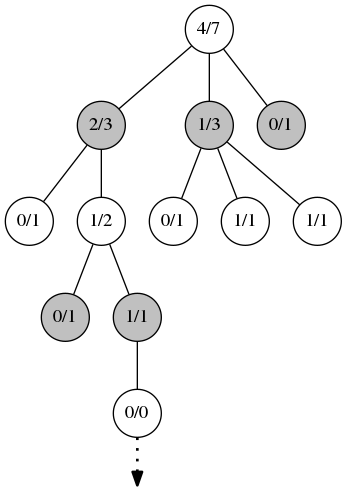
\includegraphics[width=\textwidth]{images/gametree-values}
    \caption{Game tree with values.}
    \label{fig:mcts-gametree-values}
    \end{subfigure}%
    \unskip\ \vrule\
    \begin{subfigure}{0.23\textwidth}
    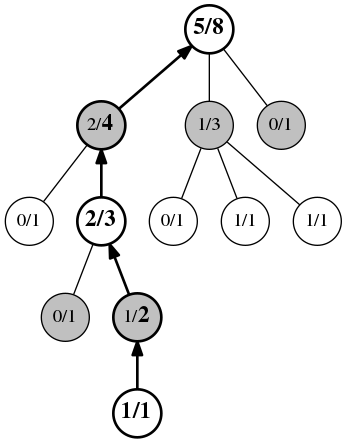
\includegraphics[width=\textwidth]{images/gametree-values-updated}
    \caption{Game tree with  updated values after win.}
    \label{fig:mcts-gametree-values-updated}
    \end{subfigure}
    \caption{MCTS Minimax game tree}
\end{figure}

\subsection{UCT}
UCT changes how MCTS selects new nodes to expand upon. In the algorithms explained above the values are only used when making the final decision as to what action to take. In other words only the values in the second layer are used. In figure \ref{fig:mcts-gametree-values-updated}, the algorithm would choose the left node with $2/4$) because it has the highest score. UCT makes a good effort to use all the intermediate values and try to spend as much time as possible in the most promising branches of the tree.
 
\subsubsection{Algorithm}
High level uitleg van het algo en idee er achter. Uitleg per 4 secties.
\subsubsection{Parameters}
Is deze nodig?
\subsubsection{Parallel}
3 verschillende manieren van MCTS parallel, en de keuze die ik gemaakt heb en waarom.
\subsubsection{Domain knowledge in simulation}
Uitleg hoe je domain knowledge in de simulation stage toevoegd. En welke ik heb toegevoegd.
\subsection{Exploration vs. Exploitation}
Uitleg over het 'traditionele' E vs E probleem.

\printbibliography

\end{document}
